\documentclass[12pt]{article}
\usepackage[utf8]{inputenc}
\usepackage[a4paper,margin=1in]{geometry}
\usepackage{amsmath} 
\usepackage{amssymb}
\usepackage{graphicx}
\usepackage{float}
\usepackage{tabularx} 
\usepackage{caption}
\usepackage{subcaption}
\usepackage{array}
\usepackage{listings}
\usepackage{pythonhighlight}



\title{
    Department Of Aerospace Engineering,\\
    Indian Institute Of Technology Madras
    \begin{figure}[H]
        \centering
        
\includegraphics[width=8cm]{iitmlogo.png}
    \end{figure}
    \begin{center}
        \textbf{\\AS2101 : Introduction to Aerospace Engineering\\}
        Report 4 : Finding the Roots of a Funtion using Bisection, Newton and Secant Method\\
    \end{center}
}
\author{
    Pranit Zope\\AE20B046
}
\date{September 28, 2021}

\begin{document}
\pagenumbering{gobble}
\maketitle
\newpage
\pagenumbering{arabic}
\tableofcontents 
\listoffigures

\newpage


\section{Aim}
We will use 3 methods namely
\begin{enumerate}
    \item Newton's Method
    \item Bisection Method
    \item Secant Method
\end{enumerate}
to find the zeroes of two given equations :
\begin{equation}
    f_1(x) = x^3-3x^2-x+9
\end{equation}
\begin{equation}
    f_2(x) = e^x f_1(x) = e^x \cdot (x^3-3x^2-x+9)
\end{equation}

\section{Theory}
\subsection{Bisection Method}
In bisection method, we will find solution by using the following steps :-
\begin{figure}[H]
    \centering
    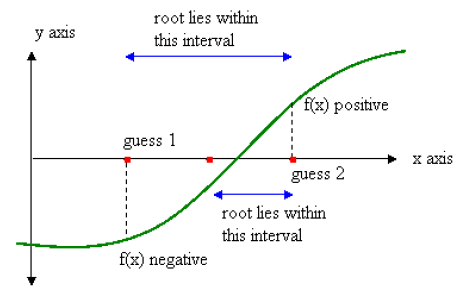
\includegraphics[width=8cm]{bis.png}
    \caption{Bisection Method}
    \label{fig:my_label}
\end{figure}
\begin{enumerate}
    \item Guess suitable a and b values such that $f(a)$ and $f(b)$ are of opposite signs, by finding images f(x) of various points and observing their trend.\\
    \item We will take a midpoint $c=\frac{a+b}{2}$ and find f(c)
    \item Here, if $f(c)\cdot f(a) > 0$ then replace b with c and repeat the process
    \item Similarly, if $f(c)\cdot f(a) < 0$ then replace a with c and repeat the process
    \item Define an $\epsilon >0$ such that $|f(c)|<\epsilon$. then $c$ will be your zero of that polynomial
\end{enumerate}
\subsection{Newton's Method}
In newton's method, we will find solution by using the following steps :-
\begin{figure}[H]
    \centering
    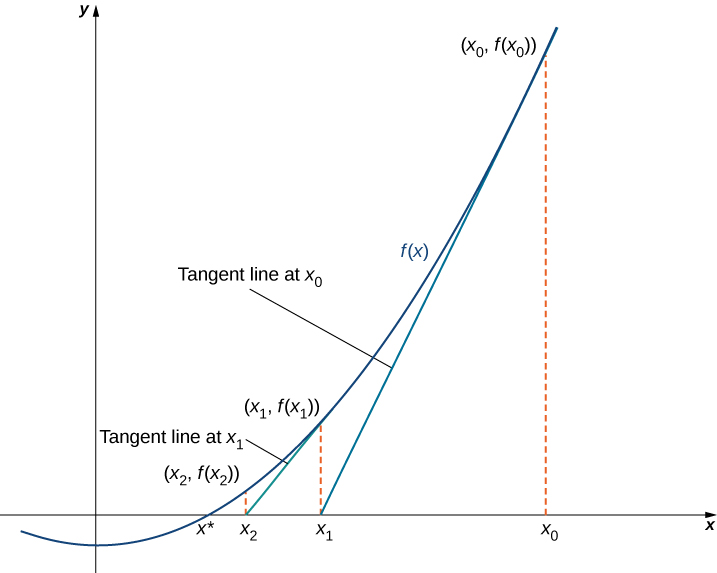
\includegraphics[width=8cm]{new.png}
    \caption{Newton's Method}
\end{figure}
\begin{enumerate}
    \item Take a random point ($x=x_0$) on the curve, and draw a tangent to it. Let it cut the X axis at a point $x_1$.
    \item \begin{equation*}
        x_n=x_{n-1} - \frac{f(x_{n-1})}{f'(x_{n-1})}
    \end{equation*}
    \item Find $y=f(x_1)$ and repeat the same for $x_2,x_3,...,x_n$
    \item Define an $\epsilon >0$ such that $|f(x_n)|<\epsilon$. then $x_n$ will be your zero of that polynomial.
\end{enumerate}
\subsection{Secant Method}
In secant method, we will find solution by using the following steps :-
\begin{figure}[H]
    \centering
    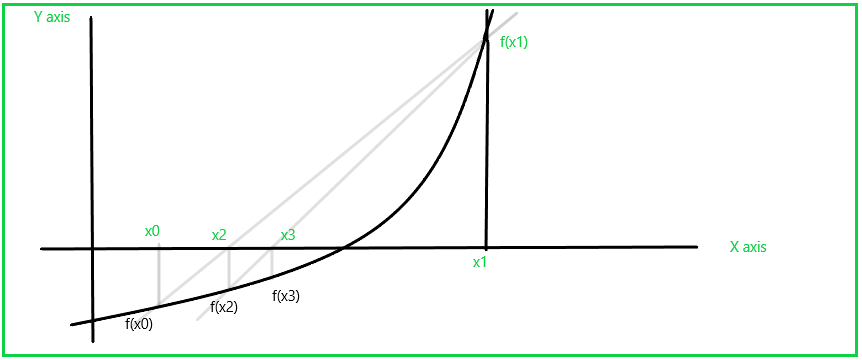
\includegraphics[width=8cm]{sec.png}
    \caption{Secant Method}
\end{figure}
\begin{enumerate}
    \item Take two points ($x=x_0$ and $x=x_1$) on the curve.
    \item Draw a secant from $f(x_0)$ and $f(x_1)$ on the curve. Let it intersect the axis at $x_2$.
    \item Repeat the same with  $f(x_2)$ and $f(x_1)$.
    \item \begin{equation*}
        x_{n+1}=x_{n-1} - \frac{f(x_{n-1})}{\frac{f(x_n)-f(x_{n-1})}{x_n - x_{n-1}}}
    \end{equation*}
    \item Define an $\epsilon >0$ such that $|f(x_n)|<\epsilon$. then $x_n$ will be your zero of that polynomial.
\end{enumerate}

\section{Graphical Analysis}
\subsection{$f_1(x)$ : Graphical Analysis by all 3 methods}
We will plot $f(x)$ vs No. of iterations plot. The plots were made using matplotlib library in python.
\subsubsection{Bisection Method}
\begin{figure}[H]
    \centering
    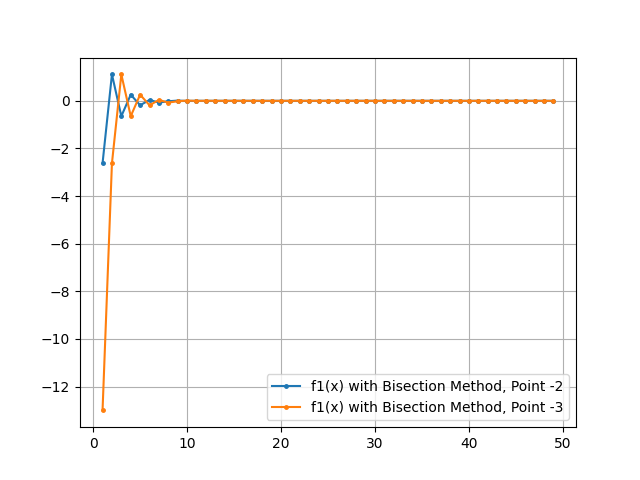
\includegraphics[width=12cm]{f1b.png}
    \caption{$f_1(x)$ vs Iterations for Bisection Method}
\end{figure}

\subsubsection{Newton's Method}
\begin{figure}[H]
    \centering
    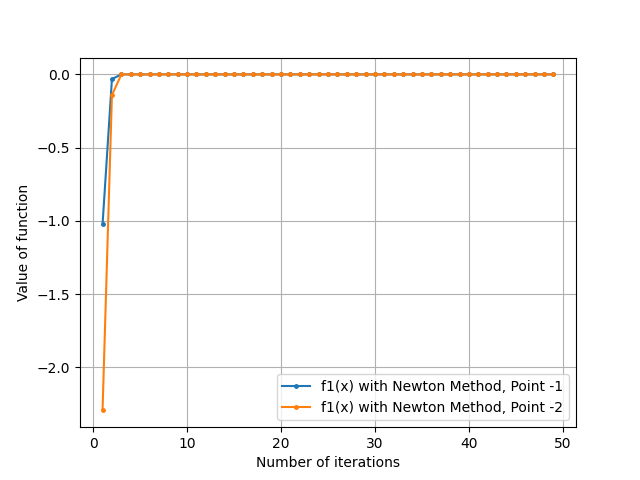
\includegraphics[width=12cm]{f1n.png}
    \caption{$f_1(x)$ vs Iterations for Newton's Method}
\end{figure}

\subsubsection{Secant Method}
\begin{figure}[H]
    \centering
    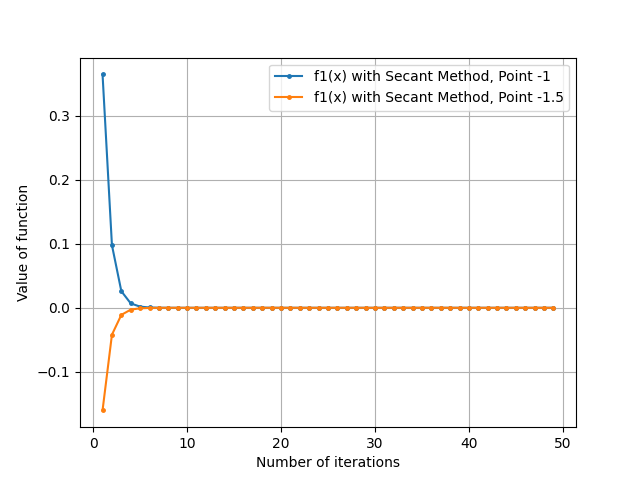
\includegraphics[width=12cm]{f1s.png}
    \caption{$f_1(x)$ vs Iterations for Secant Method}
\end{figure}

\subsubsection{Comparison of all methods}
\begin{figure}[H]
    \centering
    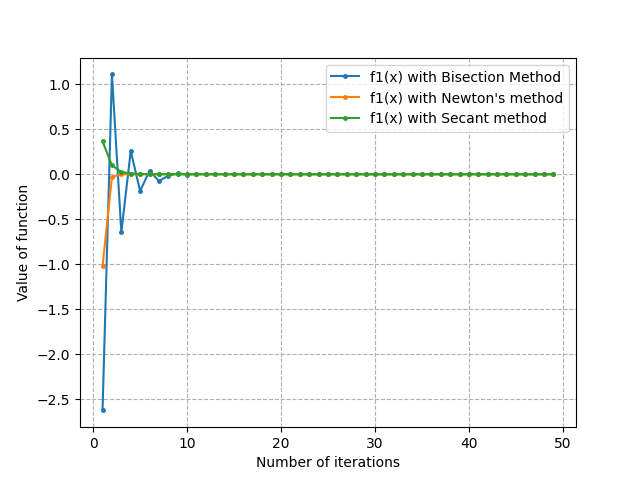
\includegraphics[width=12cm]{f1_all.png}
    \caption{$f_1(x)$ vs Iterations for All Methods side by side}
\end{figure}

\newpage
\subsection{$f_2(x)$ : Graphical Analysis by all 3 methods}
We will plot $f(x)$ vs No. of iterations plot. The plots were made using matplotlib library in python.
\subsubsection{Bisection Method}
\begin{figure}[H]
    \centering
    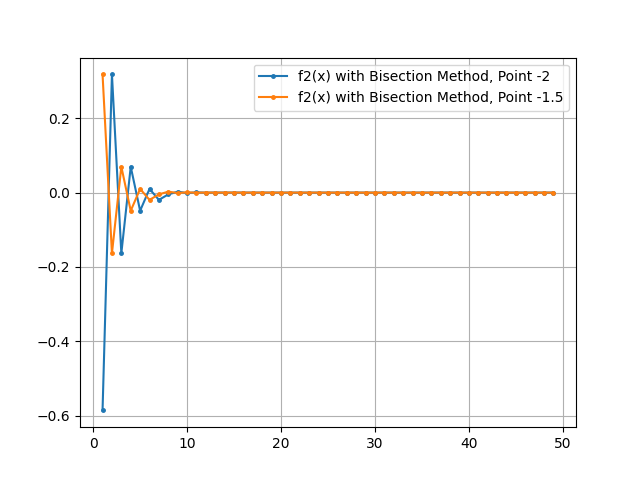
\includegraphics[width=12cm]{f2b.png}
    \caption{$f_2(x)$ vs Iterations for Bisection Method}
\end{figure}

\subsubsection{Newton's Method}
\begin{figure}[H]
    \centering
    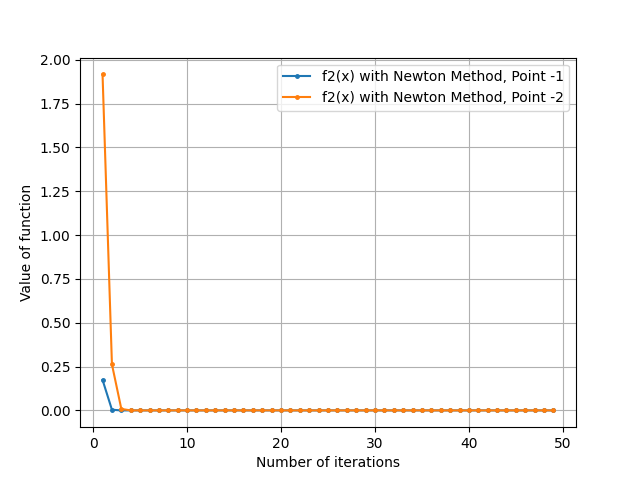
\includegraphics[width=12cm]{f2n.png}
    \caption{$f_2(x)$ vs Iterations for Newton's Method}
\end{figure}

\subsubsection{Secant Method}
\begin{figure}[H]
    \centering
    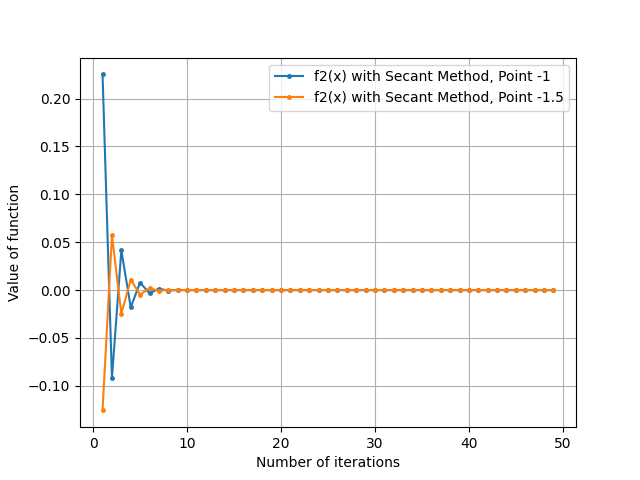
\includegraphics[width=12cm]{f2s.png}
    \caption{$f_2(x)$ vs Iterations for Secant Method}
\end{figure}

\subsubsection{Comparison of all methods}
\begin{figure}[H]
    \centering
    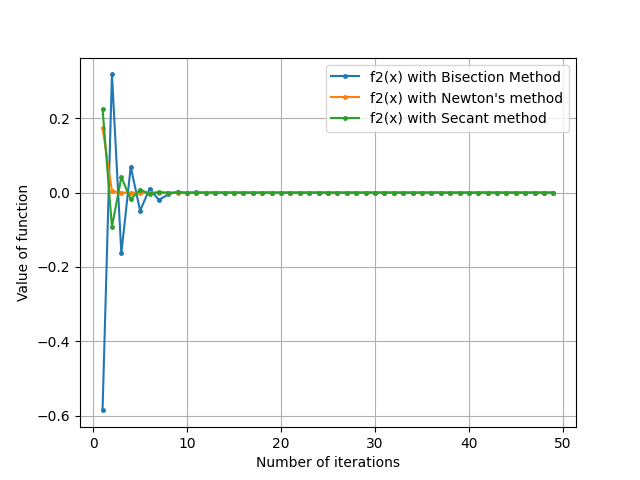
\includegraphics[width=12cm]{f2_all.png}
    \caption{$f_2(x)$ vs Iterations for All Methods side by side}
\end{figure}


\section{Results}
The following were obtained as the results :\\
First function with Bisection Method (Points : -2 and -3)\\
-1.3307456970214844\\
Second function with Bisection Method (Points : -2 and 1.5)\\
-1.3307456970214844\\
First function with Newton's method (Points : -1 and -2)\\
-1.330746086127756\\
Second function with Newton's method (Points : -1 and -2)\\
-1.3307455713782212\\
First function with Secant Method (Points : -1 and -1.5)\\
-1.3307454712328826\\
Second function with Secant Method (Points : -1 and -1.5)\\
-1.3307473010147413\\


\newpage
\section{Conclusions}
We can draw the following conclusions from the graphical analysis :
\begin{enumerate}
    \item Using computer for computing is way better than manual solving since we can solve almost all equations in a computer, whereas it isnt feasible in manual mode.
    \item We observe from the side by side comparisons that Newton's Method and the secant methods are better in comparisons to the bisection method, since the number of iterations is very large in number comparatively.
\end{enumerate}

\newpage

\appendix
\addcontentsline{toc}{section}{Appendix}

\section{Python code for computing and Plotting the roots of a mathematical function}
\begin{python}
#!/usr/bin/python3.9
# Pranit Zope
# AE20B046
# AS2101 : Assignment 04

import math
import numpy as np
import matplotlib.pyplot as plt

def f1(x):
    return (x**3-3*x**2+x+9)
def f2(x):
    return math.exp(x)*(x**3-3*x**2+x+9)

def f1dash(x):
    return (3*x**2-6*x+1)    
def f2dash(x):
    return math.exp(x)*(x**3-5*x+10)
#defined all the necessary mathematical functions which we will be needing

def bisection(f,a,b,spec=10**-12,counter=50):
    """A function that computes the root of a function in x by Bisection method.

    Args:
        f (Function): A mathematical Function in variable x
        a (float): Lower limit of calling the bisection function
        b (float): Upper limit of calling the bisection function
        spec (float, optional): The specification value upto which you want the accuracy to be maintained. Defaults to 10**-12.
        counter (int, optional): Maximum number if iterations. Defaults to 50.

    Returns:
        float: The value of the root of the function f(x).
    """

    if f(a)*f(b)>=0:
        return "Error"
    else:
        counter_index=0
        c=1
        while(abs(f(c))>spec and counter_index<counter):
            c=(a+b)/2
            if f(c)*f(b)>0:
                b=c
            if f(c)*f(a)>0:
                a=c
            counter_index+=1
        return c



def newton(f,fdash,x,spec=10**-12,counter=50):
    """A function that computes the root of a function in x by Newton method.

    Args:
        f (function):  A mathematical Function in variable x
        fdash (function):  A mathematical Function in variable x which is the derivative of f(x)
        x (float): The value at which the Newton function should be initialised.
        spec (float, optional): The specification value upto which you want the accuracy to be maintained. Defaults to 10**-12.
        counter (int, optional): Maximum number if iterations. Defaults to 50.

    Returns:
        float: The value of the root of the function f(x).
    """

    counter_index=0
    while(abs(f(x))>spec and counter_index<counter):
        counter_index+=1
        x=x-f(x)/fdash(x)
    return x



def secant(f,x0,x1,spec=10**-12,counter=50):
    """A function that computes the root of a function in x by Secant method.

    Args:
        f (function):  A mathematical Function in variable x
        x0 (float): Lower limit of calling the Secant function
        x1 (float): Upper limit of calling the Secant function
        spec (float, optional): The specification value upto which you want the accuracy to be maintained. Defaults to 10**-12.
        counter (int, optional): Maximum number if iterations. Defaults to 50.

    Returns:
        x1: The value of the root of the function f(x).
    """

    counter_index=0
    x1=x1-((x0-x1)/(f(x0)-f(x1))*f(x1))
    while(abs(f(x1))>spec and counter_index<counter):
        counter_index+=1
        x1=x1-((x0-x1)/(f(x0)-f(x1))*f(x1))
    return x1



print("First function with Bisection Method")
print(bisection(f1,-2,-1,0.00001,100))
print("Second function with Bisection Method")
print(bisection(f2,-2,-1,0.00001,100))

print("First function with Newton's method")
print(newton(f1,f1dash,-1,0.00001,100))
print("Second function with Newton's method")
print(newton(f2,f2dash,-1,0.00001,100))

print("First function with Secant Method")
print(secant(f1,-2,-1,0.00001,100))
print("Second function with Secant Method")
print(secant(f2,-2,-1,0.00001,100))
#Printing the outcomes of executing the Bisection, Newton and Secant Functions


#### SECTION TO PLOT THE FUNCTION VS ITERATION GRAPH OF f1(x) WITH ALL THE THREE METHODS ####
x=[]
y=[]
for i in range(1,50):
    x.append(i)
    y.append(f1(bisection(f1,-2,-1,counter=i)))
plt.xlabel("Number of Iterations")
plt.ylabel("Value of Function")
plt.plot(x,y,label="f1(x) with Bisection Method",marker=".",markersize="5")


x=[]
y=[]
for i in range(1,50):
    x.append(i)
    y.append(f1(newton(f1,f1dash,-1,counter=i)))
plt.xlabel("Number of iterations")
plt.ylabel("Value of function")
plt.plot(x,y,label="f1(x) with Newton's method",marker=".",markersize="5")


x=[]
y=[]
for i in range(1,50):
    x.append(i)
    y.append(f1((secant(f1,-2,-1,counter=i))))
plt.plot(x,y,label="f1(x) with Secant method",marker=".",markersize="5")
plt.grid(linestyle='--')
plt.legend()
plt.savefig("f1_all")
plt.clf()


#### SECTION TO PLOT THE FUNCTION VS ITERATION GRAPH OF f1(x) WITH ALL THE THREE METHODS ####
x=[]
y=[]
for i in range(1,50):
    x.append(i)
    y.append(f2(bisection(f2,-2,-1,counter=i)))
plt.xlabel("Number of iterations")
plt.ylabel("Value of function")
plt.plot(x,y,label="f2(x) with Bisection Method",marker=".",markersize="5")

x=[]
y=[]
for i in range(1,50):
    x.append(i)
    y.append(f2(newton(f2,f2dash,-1,counter=i)))
plt.plot(x,y,label="f2(x) with Newton's method",marker=".",markersize="5")

x=[]
y=[]
for i in range(1,50):
    x.append(i)
    y.append(f2(secant(f2,-2,-1,counter=i)))
plt.plot(x,y,label="f2(x) with Secant method",marker=".",markersize="5")
plt.grid()
plt.legend()
plt.savefig("f2_all")
plt.clf()

#### SECTION TO PLOT THE FUNCTION VS ITERATION GRAPH OF BOTH FUNCTIONS WITH BISECTION METHOD ####
x=[]
y=[]
z=[]
for i in range(1,50):
    x.append(i)
    y.append(f1(bisection(f1,-2,-1,counter=i)))
    z.append(f1(bisection(f1,-3,-1,counter=i)))
plt.plot(x,y,label="f1(x) with Bisection Method, Point -2",marker=".",markersize="5")
plt.plot(x,z,label="f1(x) with Bisection Method, Point -3",marker=".",markersize="5")
plt.grid()
plt.legend()
plt.savefig("f1b")
plt.clf()

x=[]
y=[]
z=[]
for i in range(1,50):
    x.append(i)
    y.append(f2(bisection(f2,-2,-1,counter=i)))
    z.append(f2(bisection(f2,-1.5,-1,counter=i)))
plt.plot(x,y,label="f2(x) with Bisection Method, Point -2",marker=".",markersize="5")
plt.plot(x,z,label="f2(x) with Bisection Method, Point -1.5",marker=".",markersize="5")
plt.grid()
plt.legend()
plt.savefig("f2b")
plt.clf()

#### SECTION TO PLOT THE FUNCTION VS ITERATION GRAPH OF BOTH FUNCTIONS WITH NEWTON METHOD ####
x=[]
y=[]
z=[]
for i in range(1,50):
    x.append(i)
    y.append(f1(newton(f1,f1dash,-1,counter=i)))
    z.append(f1(newton(f1,f1dash,-2,counter=i)))
plt.plot(x,y,label="f1(x) with Newton Method, Point -1",marker=".",markersize="5")
plt.plot(x,z,label="f1(x) with Newton Method, Point -2",marker=".",markersize="5")
plt.xlabel("Number of iterations")
plt.ylabel("Value of function")
plt.grid()
plt.legend()
plt.savefig("f1n")
plt.clf()

x=[]
y=[]
z=[]
for i in range(1,50):
    x.append(i)
    y.append(f2(newton(f2,f2dash,-1,counter=i)))
    z.append(f2(newton(f2,f2dash,-2,counter=i)))
plt.plot(x,y,label="f2(x) with Newton Method, Point -1",marker=".",markersize="5")
plt.plot(x,z,label="f2(x) with Newton Method, Point -2",marker=".",markersize="5")
plt.xlabel("Number of iterations")
plt.ylabel("Value of function")
plt.grid()
plt.legend()
plt.savefig("f2n")
plt.clf()


#### SECTION TO PLOT THE FUNCTION VS ITERATION GRAPH OF BOTH FUNCTIONS WITH SECANT METHOD ####
x=[]
y=[]
z=[]
for i in range(1,50):
    x.append(i)
    y.append(f1(secant(f1,-2,-1,counter=i)))
    z.append(f1(secant(f1,-2,-1.5,counter=i)))
plt.plot(x,y,label="f1(x) with Secant Method, Point -1",marker=".",markersize="5")
plt.plot(x,z,label="f1(x) with Secant Method, Point -1.5",marker=".",markersize="5")
plt.xlabel("Number of iterations")
plt.ylabel("Value of function")
plt.grid()
plt.legend()
plt.savefig("f1s")
plt.clf()

x=[]
y=[]
z=[]
for i in range(1,50):
    x.append(i)
    y.append(f2(secant(f2,-2,-1,counter=i)))
    z.append(f2(secant(f2,-2,-1.5,counter=i)))
plt.plot(x,y,label="f2(x) with Secant Method, Point -1",marker=".",markersize="5")
plt.plot(x,z,label="f2(x) with Secant Method, Point -1.5",marker=".",markersize="5")
plt.xlabel("Number of iterations")
plt.ylabel("Value of function")
plt.grid()
plt.legend()
plt.savefig("f2s")
plt.clf()

\end{python}

\end{document}
